\documentclass[usenames,dvipsnames,aspectratio=169]{beamer}
\usepackage[utf8]{inputenc}
\usepackage[spanish]{babel}
\usepackage{csquotes}
\usepackage[skip=0pt]{caption}
\captionsetup[figure]{labelformat=empty}
\usepackage{booktabs}
\usepackage{tabularx, colortbl}
\usepackage{setspace}
\usepackage{hyperref}
\usetheme{uniud}

%%% Some useful commands
% pdf-friendly newline in links
\newcommand{\pdfnewline}{\texorpdfstring{\newline}{ }} 
% Fill the vertical space in a slide (to put text at the bottom)
\newcommand{\framefill}{\vskip0pt plus 1filll}
\renewcommand{\emph}[1]{\textbf{\textcolor{UniGold}{#1}}}


\title[]{{\Large Sistemas Inteligentes\\CLIPS}\\[0.2cm]Tema 1: Introducción}

\date[Marzo, 2022]{Marzo de 2023}
\author[Aurora Esteban]{\texorpdfstring{
    \begin{minipage}{0.47\linewidth}
        Aurora Esteban Toscano
        \pdfnewline
        \texttt{aestebant@uco.es}
    \end{minipage}
    \hfill
    \begin{minipage}{0.47\linewidth}
        José Manuel Alcalde Llergo
        \pdfnewline
        \texttt{i72alllj@uco.es}
    \end{minipage}
}{Aurora Esteban Toscano}
}
\institute{Grado en Ingeniería Informática, Universidad de Córdoba}

\begin{document}

\begin{frame}
\titlepage
\end{frame}

\begin{frame}{Objetivos}
	\begin{itemize}
		\item Introducir los Sistemas Expertos.
		\item Instalar CLIPS.
		\item Familiarizarse con el entorno de CLIPS.
	\end{itemize}
\end{frame}

\begin{frame}{Sistemas basados en reglas}
Los \textbf{Sistemas basados en reglas} son mecanismos para representar el conocimiento con reglas de tipo \texttt{si-entonces} o \texttt{if-then}.
\begin{itemize}
	\item También pueden conocerse como Sistemas de Producción.
\end{itemize}
\begin{exampleblock}{Por ejemplo}
	\texttt{SI} es de noche, \texttt{ENTONCES} enciende la luz.
\end{exampleblock}
Una aplicación fundamental son los \textbf{Sistemas Expertos}: sistemas que buscan emular la toma de decisiones de un experto humano para resolver problemas complejos $\rightarrow$ una de las formas más populares de \textit{Inteligencia Artificial}.
\end{frame}

\begin{frame}{Sistemas Expertos (basados en reglas) I}
	Los Sistemas Expertos son capaces de llegar a un diagnóstico aplicando reglas de forma encadenada sobre un conjunto de datos por medio de los siguientes componentes:
	\begin{itemize}
		\item \textbf{Base de conocimientos:} almacena las reglas previamente definidas $\rightarrow$ conocimiento estático.
		\item \textbf{Base de afirmaciones:} almacena los hechos sobre los que trabajan las reglas $\rightarrow$ conocimiento dinámico.
		\item \textbf{Motor de inferencia:} aplica las reglas a los hechos para deducir nuevos hechos.
		\item \textbf{Interfaz de usuario:} permite introducir la información de partida, seguir el proceso de razonamiento o inferencia y obtener el diagnóstico final.
	\end{itemize}
\end{frame}

\begin{frame}{Sistemas Expertos (basados en reglas) II}
	\begin{exampleblock}{Por ejemplo}
		Base de conocimientos:
		\begin{itemize}
			\item Todos los hombres son animales.
			\item Todos los animales respiran.
		\end{itemize}
		Base de afirmaciones:
		\begin{itemize}
			\item Juan es un hombre.
		\end{itemize}
		Inferencia:
		\begin{enumerate}
			\item Juan es un animal.
			\item Juan respira.
		\end{enumerate}
	\end{exampleblock}
\end{frame}

\begin{frame}{Estructura de las reglas}
	\begin{block}{Dos partes fundamentales}
		\centering
		\textbf{Antecedente} $\Longrightarrow$ \textbf{Consecuente}
	\end{block}
	\begin{itemize}
		\item Antecedente: cero o más \textit{cláusulas} que deben cumplirse para que la regla pueda ejecutarse (dispararse).
		\item Consecuente: cero o más \textit{acciones} que se llevarán a cabo si la regla se dispara.
		\begin{itemize}
			\item Entre esas acciones puede estar crear (afirmar) más hechos, eliminar hechos obsoletos, llegar a conclusiones finales...
		\end{itemize}
	\end{itemize}
	\begin{exampleblock}{Por ejemplo}
		\centering
		\texttt{SI} voy a clase \texttt{Y} atiendo \texttt{Y} hago los ejercicios $\Longrightarrow$ apruebo la asignatura
	\end{exampleblock}
\end{frame}

\begin{frame}{Inferencia I}
	El motor de inferencia determina cómo se pasa de los hechos al conocimiento.
	\begin{itemize}
		\item Las reglas se ejecutan hacia adelante: si se satisface el antecedente se efectúan las acciones del consecuente.
		\item Un grupo de reglas que contienen un problema y una solución se llama cadena:
		\begin{itemize}
			\item Encadenamiento hacia delante o basado en datos: va desde los hechos iniciales, pasando por hechos inferidos y acabando en una conclusión.
			\begin{itemize}
				\item \textbf{Nos centraremos en este.}
			\end{itemize}
			\item Encadenamiento hacia atrás o basado en objetivos: parte de una hipótesis objetivo que deberá probarse mediante hipótesis intermedias que deberán estar sostenida por hechos.
		\end{itemize}
	\end{itemize}
\end{frame}

\begin{frame}{Inferencia II}
	El \textbf{Control de razonamiento} es un mecanismo del motor de inferencia que se encarga de seleccionar \textit{qué regla disparar si hay varias disponibles}.
	
	Métodos de resolución de conflictos:
	\begin{enumerate}
		\item Ordenación de las reglas.
		\item Ordenar las cláusulas dentro de cada regla.
		\item Añadir nuevas cláusulas relacionadas con las inferencias.
		\item Control mediante agenda.
		\item Agendas con patrocinadores.
		\item Conjuntos de reglas.
		\item Modelos de reglas y metarreglas.
		\item Mecanismos basados en la sensibilidad y estabilidad del sistema.
	\end{enumerate}
\end{frame}

\begin{frame}{CLIPS}
	CLIPS (\textit{\textbf{C} \textbf{L}anguage \textbf{I}ntegrated \textbf{P}roduction \textbf{S}ystem}) es una herramienta para el desarrollo de Sistemas Expertos.
	\begin{itemize}
		\item Originada en 1986, \textit{NASA Software Technology Branch}.
		\item En la actualidad va por la versión 6.40, de abril de 2021.
		\item Proyecto: \url{https://sourceforge.net/projects/clipsrules/}
	\end{itemize}
	\begin{figure}
		
\includegraphics[width=0.3\linewidth]{graphics/clips_logo.png}
	\end{figure}
\end{frame}

\begin{frame}{Instalación de CLIPS I}
	Desde la página del proyecto: \texttt{Files > CLIPS > 6.40}
	\begin{figure}
		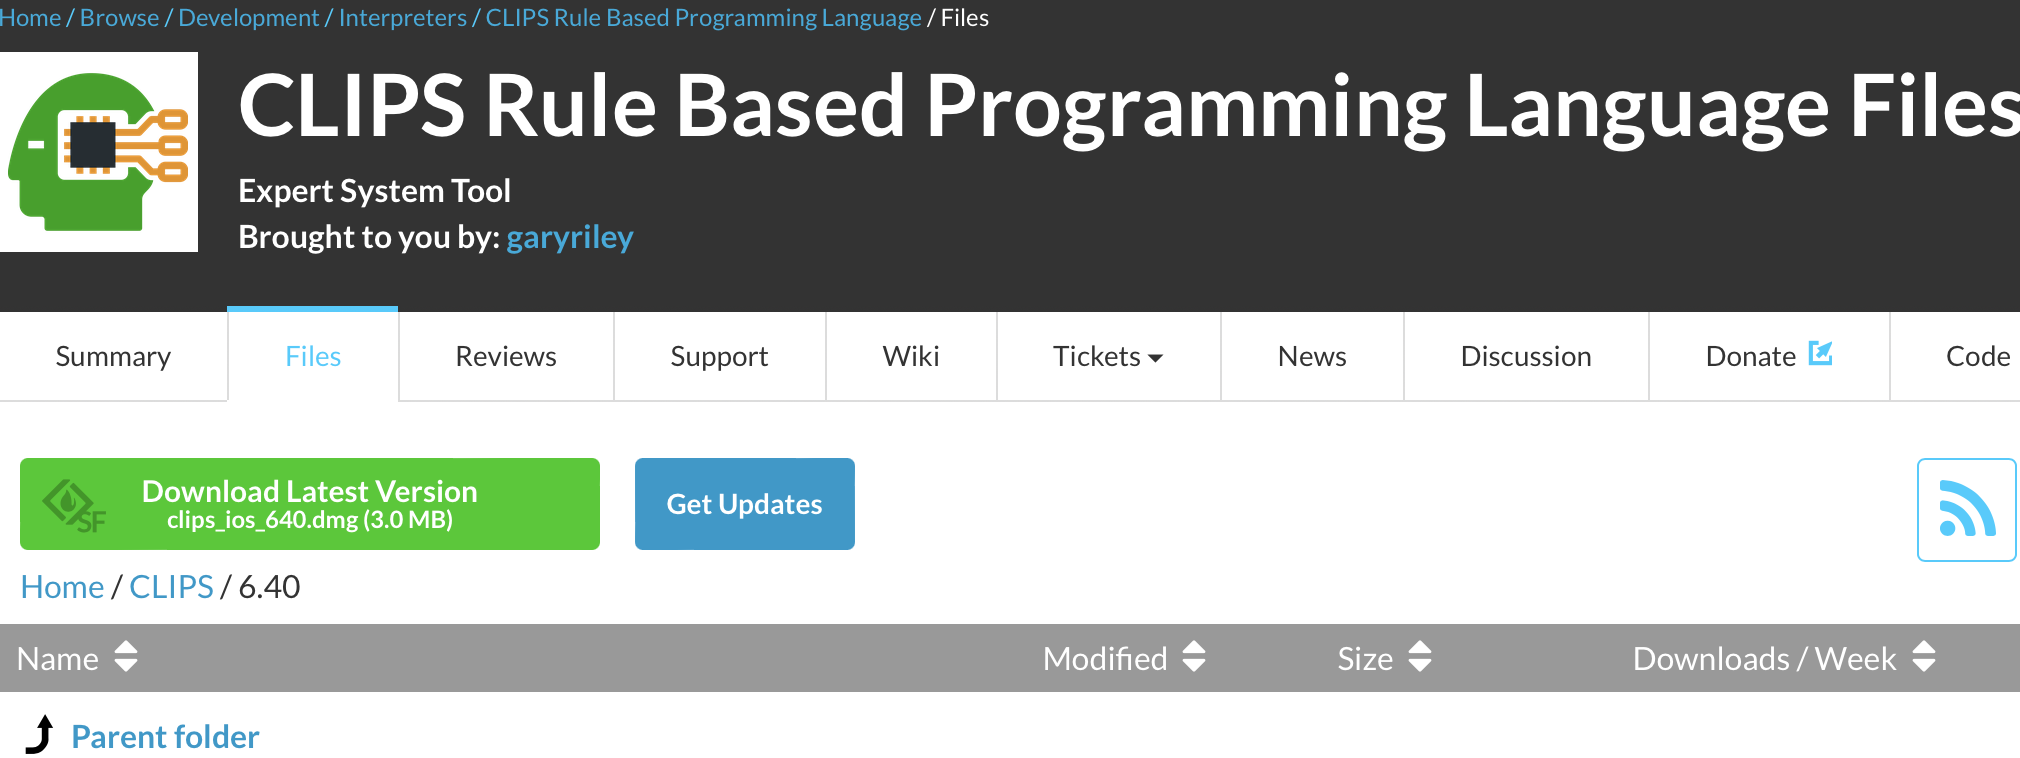
\includegraphics[width=.7\linewidth]{graphics/clips_descarga.png}
	\end{figure}
\end{frame}

\begin{frame}{Instalación de CLIPS II}
	Según tu sistema operativo:
	\begin{itemize}
		\item Windows: \texttt{clips\_windows\_64\_bit\_installer\_640.msi} y seguir el asistente.
		\item MacOS: \texttt{clips\_macos\_executable\_640.dmg} y seguir el asistente.
		\item Linux: \texttt{clips\_jni\_640.zip} (requiere Java)
		\begin{enumerate}
			\item Compilar la librería en \texttt{CLIPSJNI/library-src}: \texttt{make -f makefile.lnx <dist>}
			\begin{itemize}
				\item Posibles: ubuntu, fedora, debian, mint, centos 
			\end{itemize}
			\item Copiar \texttt{libCLIPSJNI.so} a la raíz de la carpeta de instalación
			\item Ejecutar \texttt{java -Djava.library.path=. -jar CLIPSIDE.jar}
		\end{enumerate}
		\item Sistema UCO Thinstation: ya está instalado.
	\end{itemize}
\end{frame}

\begin{frame}{Interfaz de CLIPS}
	\begin{figure}
		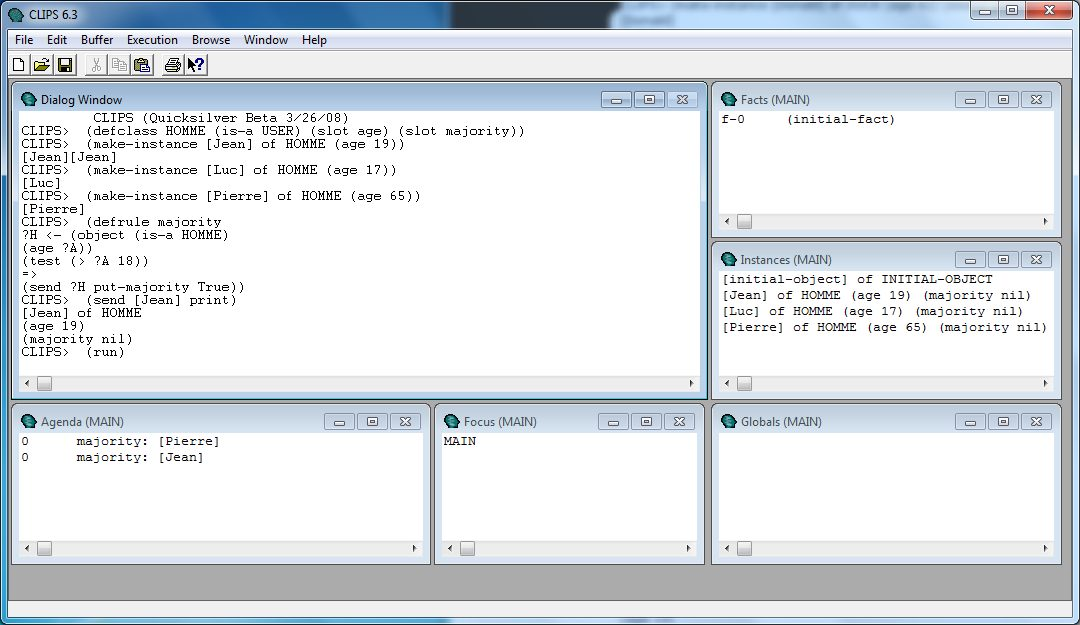
\includegraphics[width=.85\linewidth]{graphics/clips_screen}
	\end{figure}
\end{frame}

\begin{frame}{Arquitectura de CLIPS}
	\begin{itemize}
		\item Memoria de Trabajo \texttt{(facts)}: memoria global que contiene los hechos \texttt{(fact-list)} que representan el conocimiento que el sistema ha adquirido del problema particular que intenta resolver.
		\item Base de reglas \texttt{(knowledge base)}: contiene las reglas que representan el conocimiento general de resolución de problemas.
		\item Intérprete \texttt{(inference engine)}: controla la ejecución global de las reglas.
		\begin{itemize}
			\item CLIPS es un programa dirigido por los hechos $\rightarrow$ encadenamiento hacia delante.
		\end{itemize}
	\end{itemize}
\end{frame}

\begin{frame}{Documentación oficial de CLIPS}
	\begin{itemize}
		\item CLIPS Reference Manual
		\begin{itemize}
			\item Volumen I. The Basic Programming Guide.
			\item Volumen II. The Advanced Programming Guide.
			\item Volumen III. The Interfaces Guide.
		\end{itemize}
		\item CLIPS User's Guide.
	\end{itemize}
	\begin{block}{Descarga (comprobar que es la versión 6.40)}
		\url{https://sourceforge.net/projects/clipsrules/files/CLIPS/6.40/clips_examples_640.zip/download}
	\end{block}
	\begin{itemize}
		\item Ayuda de CLIPS: Menú \texttt{Help > CLIPS HELP}
		\begin{itemize}
			\item Contenido: sumario de comandos, constructores, funciones.
			\item Índice: para buscar por palabra.
		\end{itemize}
	\end{itemize}
\end{frame}

\begin{frame}{CLIPS: Primer ejemplo}
	Abrir el fichero \texttt{hombre.clp} (descarga de Moodle).
	\begin{itemize}
		\item Base de conocimiento: 2 reglas: \texttt{r-hombre-animal} y \texttt{r-animal-respira}
		\item Base de afirmaciones: Juan
		\item Fíjate en el uso de variables.
		\item Carga las reglas y afirma el hecho.
		\item Fíjate en la ventana de hechos y/o ejecuta \texttt{(facts)}
		\item Fíjate en la ventana de agenda y/o ejecuta \texttt{(agenda)}
		\item Ejecuta \texttt{(run)} para disparar el motor de inferencia.
	\end{itemize}
\end{frame}

\begin{frame}{Elementos básicos de programación}
	\begin{itemize}
		\item \textbf{Tipos de datos:} representan información.
		\item \textbf{Funciones:} manipular los datos.
		\item \textbf{Constructores:} añadir conocimiento a la Base de Conocimiento.
		\item \textbf{Comentarios:} añadir interpretabilidad a la información representada.
	\end{itemize}
\end{frame}

\begin{frame}{CLIPS: tipos de datos I}
	Tipos de datos primitivos:
	\begin{itemize}
		\item \texttt{INTEGER}: número entero. Por ejemplo: 23125, +89, -71
		\item \texttt{FLOAT}: número real. Por ejemplo: 46.5, -3.14, 45e5, +1e10
		\item \texttt{SYMBOL}: símbolo. Por ejemplo: Hola, hola, DNI34321E, coche\_rojo
		\item \texttt{STRING}: cadena. Por ejemplo: ``coche rojo'', ``carácter \textbackslash`` especial escapado''
		\item \texttt{EXTERNAL-ADDRESS}: dirección externa.
		\item \texttt{FACT-ADDRESS}: dirección de hecho.
		\item Nombre de instancia
		\item \texttt{INSTANCE-ADDRESS}: dirección de instancia.
	\end{itemize}
\end{frame}

\begin{frame}{CLIPS: tipos de datos II}
	Tipos de campos:
	\begin{itemize}
		\item \textbf{Monocampo:} está compuesto de un valor primitivo. Por ejemplo: Perro, 45, "Juan Manuel"
		\item \textbf{Multicampo:} está compuesto de cero o más valores primitivos agrupados entre paréntesis. Por ejemplo: (), (Perro), (Perro, 45, "Juan Manuel")
	\end{itemize}
	Valores de los campos:
	\begin{itemize}
		\item \textbf{Constante:} (Perro, 45, "Juan Manuel")
		\item \textbf{Variable:}
		\begin{itemize}
			\item \texttt{?<nombre>}: referencia a un monocampo. Ámbito local.
			\item \texttt{\$?<nombre>}: referencia a un multicampo. Ámbito local.
			\item \texttt{?*<nombre>*}: referencia a un monocampo o a un multicampo. Ámbito global.
		\end{itemize}
	\end{itemize}
\end{frame}

\begin{frame}{CLIPS: funciones}
	Tipos:
	\begin{itemize}
		\item Órdenes: ejecutan una acción.
		\item Funciones: devuelven un valor.
	\end{itemize}
	Definición:
	\begin{itemize}
		\item Del sistema. Por ejemplo:
		\begin{itemize}
			\item Tipos de datos: \texttt{integerp}, \texttt{floatp}, \texttt{numberp}, \texttt{symbolp}, \texttt{stringp}, \texttt{lexemep}
			\item Booleana: \texttt{eq}, \texttt{neq}, \texttt{and}, \texttt{or}, \texttt{not}
			\item Lógica mates: \texttt{=}, \texttt{<>}, \texttt{<}, \texttt{<=}, \texttt{>}, \texttt{>=}
			\item Operaciones: \texttt{+}, \texttt{-}, \texttt{*}, \texttt{/}, \texttt{div}, \texttt{mod}, \texttt{sqrt}, \texttt{**}, \texttt{round}, \texttt{abs}, \texttt{max}, \texttt{min}
		\end{itemize}
		\item Definidas por el usuario
	\end{itemize}
	\begin{block}{\small Llamada mediante notación prefija}
		\small
		\texttt{(funcion argumentos+)}
		
		\texttt{(+ (* 3 4 ) 8)}
	\end{block}
\end{frame}

\begin{frame}{CLIPS: construcctores}
	Modifican el entorno de CLIPS.
	\begin{itemize}
		\item \texttt{defmodule}: agrupar base de conocimiento en módulos.
		\item \texttt{defrule}: definir reglas.
		\item \texttt{deffacts}: afirmar hechos que se afirmarán cada vez que se reinicie el sistema.
		\item \texttt{deftemplate}: definir plantillas para hechos.
		\item \texttt{defglobal}: definir variables globales.
		\item \texttt{deffunction}: crear funciones.
		\item \texttt{defgeneric}: crear funciones genéricas.
	\end{itemize}
\end{frame}

\begin{frame}{CLIPS: comentarios}
	Dos modalidades:
	\begin{itemize}
		\item Documentación por defecto: en todos los constructores (excepto \texttt{defglobal}) a continuación del nombre del constructor y entre comillas.
	\end{itemize}
	\begin{exampleblock}{Por ejemplo}
		\texttt{(defrule regla-1 ``Regla de prueba'' a $\Rightarrow$ b)}
	\end{exampleblock}
	\begin{itemize}
		\item Comentario de lína: en cualquier parte del código comenzando por punto y coma.
	\end{itemize}
	\begin{exampleblock}{Por ejemplo}
		\texttt{; Esto es un comentario}
	\end{exampleblock}
\end{frame}

\begin{frame}
\titlepage
\end{frame}
\end{document}